\documentclass{article}
\title{Notes for: Variational Intrinsic Control}
\author{M. Nef. \thanks{paper: https://arxiv.org/abs/1611.07507}}
\date{\today}
\usepackage{amsmath}
\usepackage{amsfonts}
\usepackage[margin=1in]{geometry}
\usepackage{tikz}
\usepackage{pgfplots}
\usetikzlibrary{calc}
\usepackage{graphicx}
\DeclareMathOperator*{\argmax}{arg\,max}
\DeclareMathOperator*{\argmin}{arg\,min}

\begin{document}
\maketitle

\section{Preliminaries}

\subsection{What are ``options''}

An option is a procedure which can be executed by an agent. Once an option has been executed it will take actions for the agent and eventually, at some point, return control back to the agent. In other words: It's some policy with a termination condition.


An option itself is not a policy, an option, \(\in \Omega\) (all possible options), is just some element in the \(\Omega\) space.
A policy for a particular option is defined as:
\begin{equation}
  \label{eq:1}
  \pi(a | s, \Omega)
\end{equation}

This comes to be important, since, depending on how we define \(\Omega\) we will be able to look at how similar different options are.


When an option's policy is executed, the current state the agent is initially in is denoted \(s_{0}\). The final state the agent is in when the option's policy returns control is denoted \(s_{f}\).


In this paper, they say two options are identical if when both starting in \(s_{0}\) they both reach the same terminal state \(s_{f}\).


\begin{figure}[!ht]
\begin{center}
  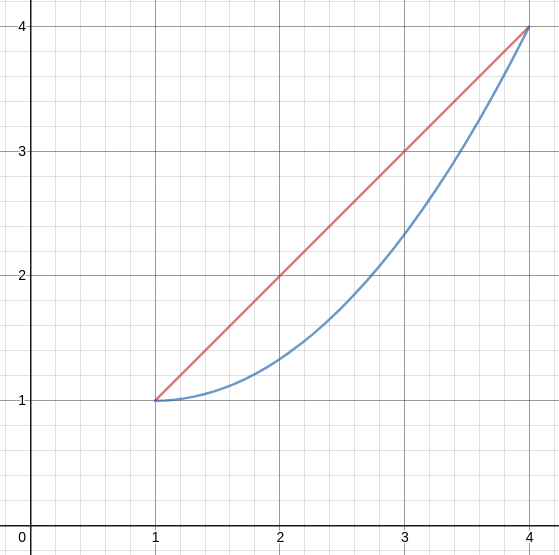
\includegraphics[width=60mm]{images/same_options.png}
  \caption{Two options which are considered the same. both start at (1,1) and terminate at (4,4) however their path is different.}
\end{center}
\end{figure}

\pagebreak
Additionally, there are 2 types of options. {\bf Closed loop} options, and {\bf Open loop} options.
\paragraph{Open Loop} options are where you select a sequence of actions to execute and the agent then blindly follows this pre-decided sequence (regardless of new observations).
\paragraph{Closed Loop} options are where you run a policy conditioned on the option representation. This allows the agent to respond to changes in the environment.

\section{Body}

They create an algorithm to generate as many {\bf different options} for an agent as possible. Each of these options should terminate at a different location to all of the others. These options can then be executed by the agent to either maximise reward or maximise ``empowerment'' (which is basically a measure of an agent's ability to reach new states from the current state).





\end{document}
